\section{Introducere}
\begin{figure}[h]
	\centering
	\begin{subfigure}[b]{0.3\textwidth}
		\centering
        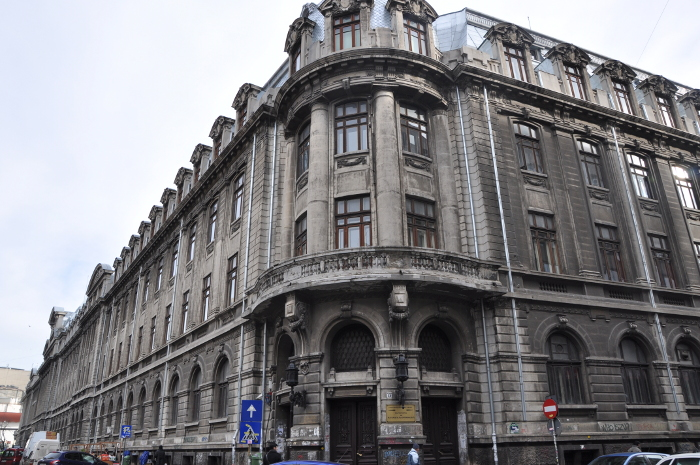
\includegraphics[height=5cm, width=\textwidth]{content_unibuc}
        \label{fig:content_unibuc}
	\end{subfigure}
    \hfill
    \begin{subfigure}[b]{0.3\textwidth}
		\centering
        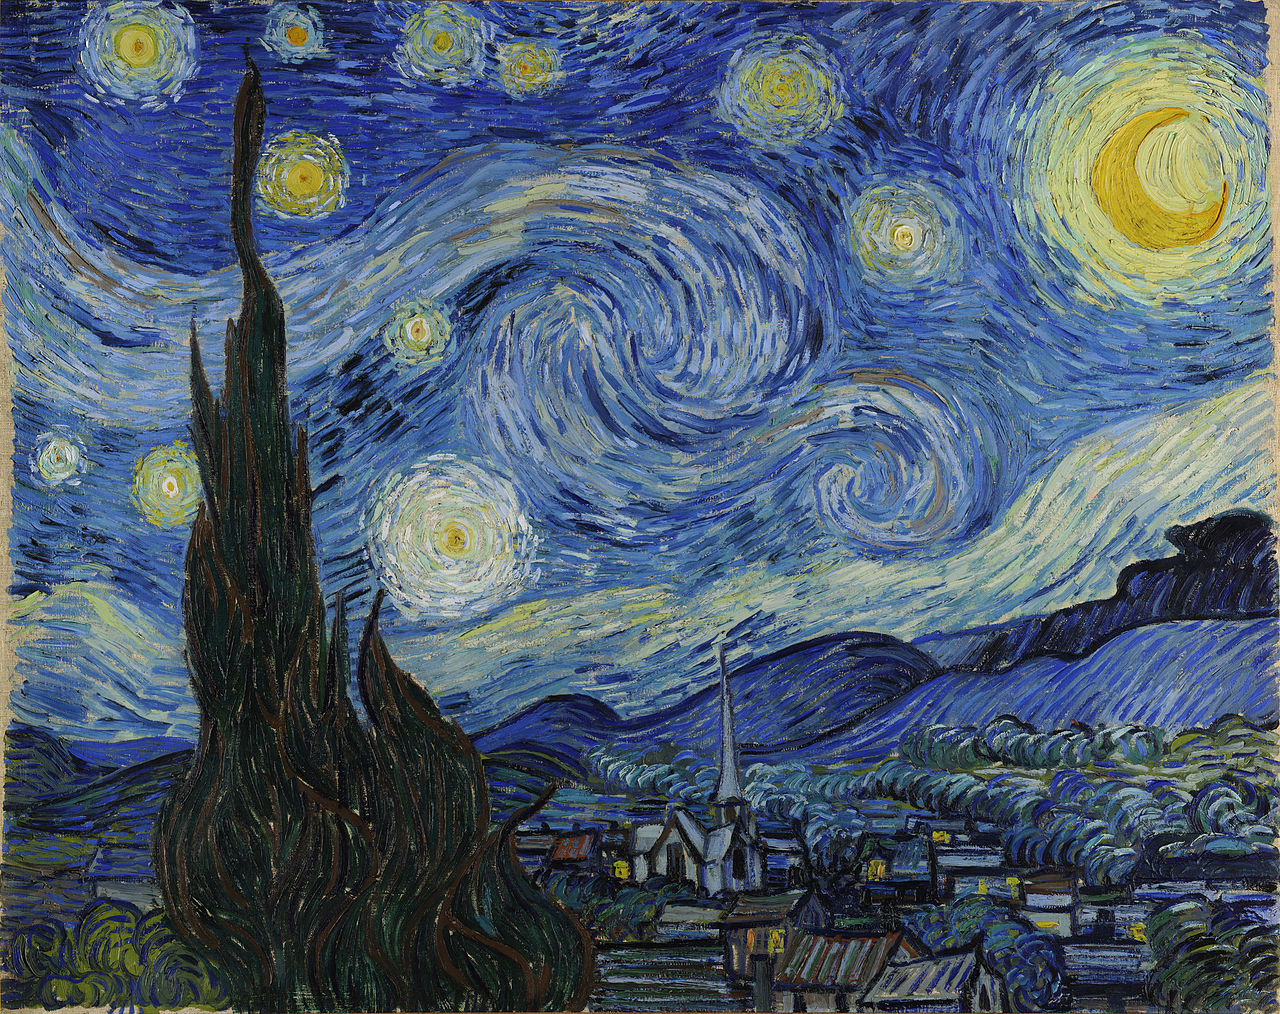
\includegraphics[height=5cm, width=\textwidth]{style1}
        \label{fig:style_unibuc}
	\end{subfigure}
    \hfill
    \begin{subfigure}[b]{0.3\textwidth}
		\centering
        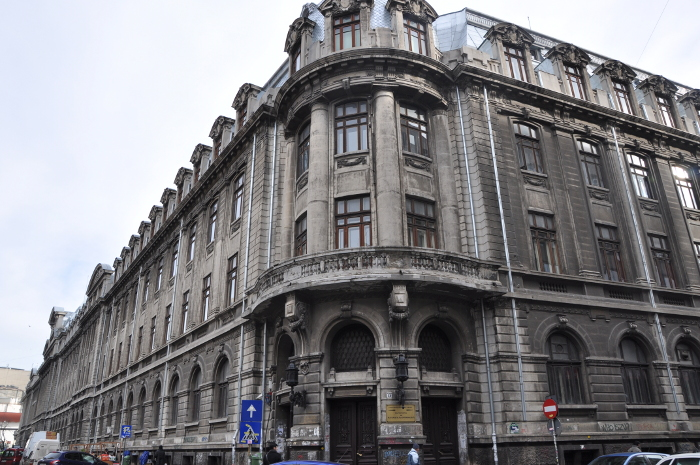
\includegraphics[height=5cm, width=\textwidth]{unibuc}
        \label{fig:content_style_unibuc}
	\end{subfigure}
    \label{fig:unibuc}
\end{figure}

	De-a lungul timpului, oamenii au reușit să altereze mediul înconjurător combinând diferite obiecte cu anumite stiluri, fie ele abstracte sau mai apropiate de realitate, obținând astfel opere de artă. Deși această acțiune este ușor de realizat de către oameni, fiind făcută chiar și de copii, este dificil să se găsească un algoritm care să simuleze acest proces deoarece creierul uman este complex, modul în care funcționează nefiind înțeles în totalitate de către oameni.

\section{Prezentarea lucrării}
În cele ce urmează o să prezint o modalitate pentru rezolvarea problemei din introducere, aceea de a combina conținutul unei poze cu stilul altei poze, obținând astfel poze artistice, asemănătoare cu cele create de om \cite{gatys2015}. Apoi, la această metodă voi adăuga noi constrângeri pentru a putea crea poze cât mai fotografice, de a putea schimba o poză din zi în noapte, de a schimba anotimpul din poză, etc \cite{luan2017}. În final, o să prezint o metodă pentru ca poza dorită să fie creată în timp real deoarece pentru a obține o poză cu metodele anterioare este necesar un timp mai mare de rulare \cite{johnson2016}.

Metodele de mai sus sunt posibile cu ajutorul învățării automate, termen care a fost inventat de către Arthur Samuel în 1959 și care a spus despre învățarea automată: "Un domeniu de studiu care oferă calculatorului abilitatea de a învăța fără a fi explicit programat.", mai exact cu ajutorul rețelelor neurale convoluționale (CNN) [\ref{fig:cnn}]. Având o poză inițializată cu un zgomot aleator sau chiar cu poza în care se află conținutul și o funcție de cost definită pe baza celor trei poze, poza inițială, poza cu conținut și poza cu stil, se vor modifica pixelii din poza inițială astfel încât costul să fie cât mai mic și astfel se va obține o poză artistică având conținutul pozei cu conținut și stilul pozei cu stil.

\begin{figure}[H]
	\centering
	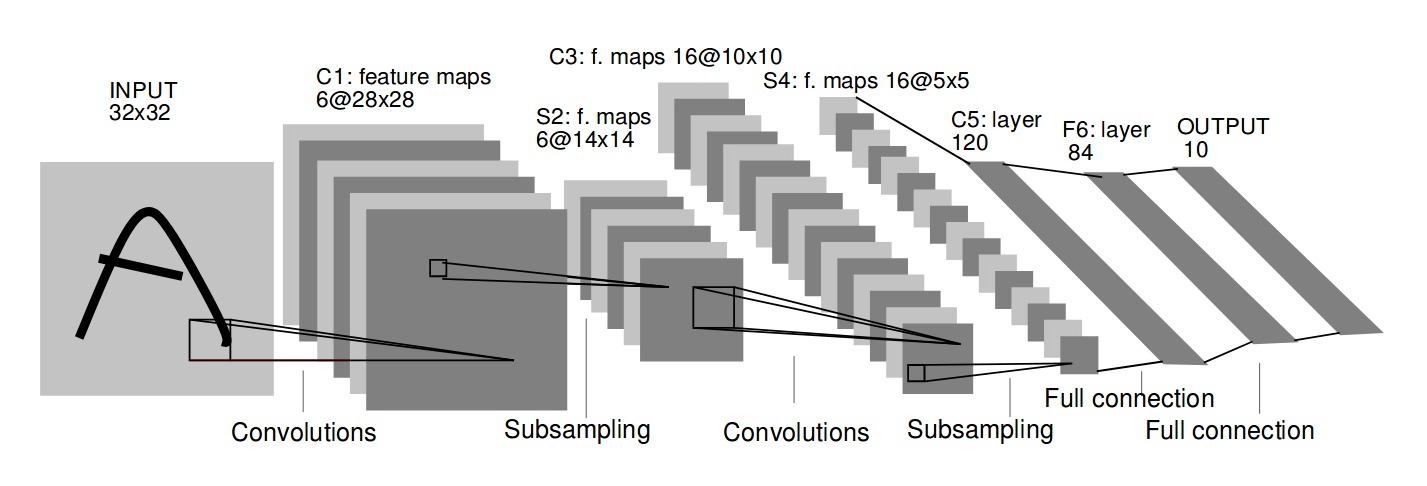
\includegraphics[height=6cm, width=\textwidth]{cnn}
	\caption{Rețea neurală convoluțională \cite{lecun-98}}
	\label{fig:cnn}
\end{figure}

În figura [\ref{fig:cnn}] este prezentă arhitectura unei rețele neurale convoluționale. Acest tip de rețele au adus o îmbunătățire semnificativă în rezolvarea problemelor cu imagini.

Modul în care această rețea merge este unul simplu. La fiecare layer, numit layer convoluțional, sunt definite așa numitele filtre sau kernele de o anumită dimensiune, această dimensiune reprezintă cât de mare este porțiunea din imagine pe care o vede un anumit filtru. Acest filtru, este plimbat pe imagine, de-a lungul tuturor canalelor imaginii, din $n$ în $n$ pixeli și fiecare valoare din filtru este înmulțită cu pixelul corespunzător din porțiunea din imagine, iar apoi aceste valori sunt adunate pentru a obține un singur număr, activarea neuronului. Numerele respective sunt puse într-o matrice ce poartă denumirea de matricea activărilor. Descrierea anterioară se poate vedea mai bine în figura [\ref{fig:filters}].

\begin{figure}[H]
	\centering
	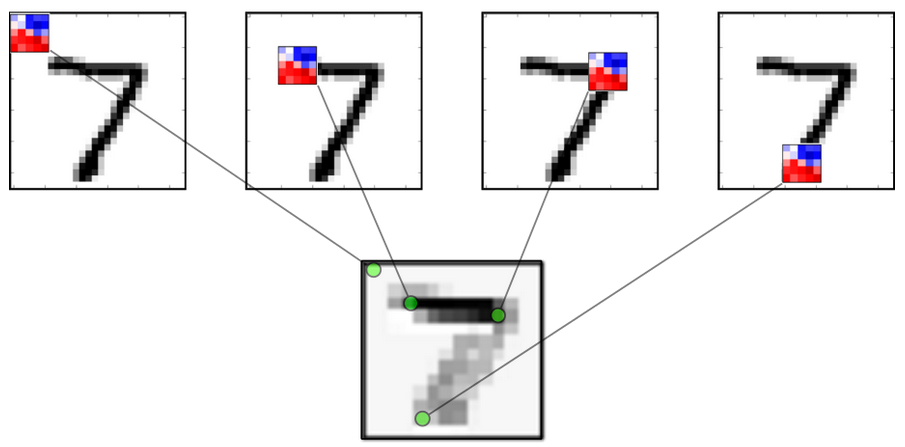
\includegraphics[height=6cm, width=\textwidth]{filters}
	\caption{\cite{filters}}
	\label{fig:filters}
\end{figure}

La un anumit layer există mai multe filtre, fiecare având anumite activări, iar aceste activări sunt așezate ca într-o stivă, precum se poate observa și în figura [\ref{fig:cnn}]. Peste aceste activări este aplicată o funcție neliniară, de obicei ReLU [\ref{sb:relu}] și apoi sunt date ca intrare la următorul layer. Pentru ca rețeaua să învețe caracteristici mai complexe este nevoie ca imaginea inițială să fie micșorată pe parcursul rețelei. Pentru a micșora imaginea sunt posibile mai multe variante, o variantă este de a folosi un tip de layer numit pooling layer. Acesta se bazează pe plimbarea unei ferestre de o anumită dimensiune pe imagine, iar din toți pixelii aflați în fereastră se obține un singur număr reprezentând valoarea maximă a pixelilor sau media tuturor pixelilor [\ref{fig:pool_layer}].

\begin{figure}[h]
	\centering
	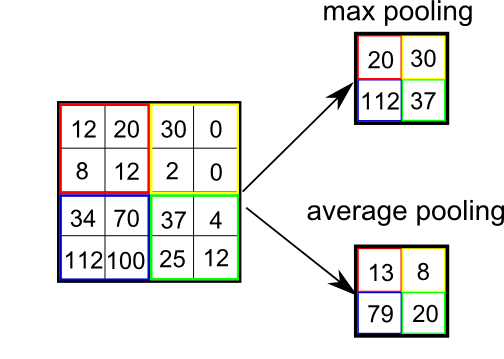
\includegraphics[height=8cm, width=\textwidth]{pool_layer}
	\caption{\cite{pooling}}
	\label{fig:pool_layer}
\end{figure}

O altă variantă de micșorare a pozei este aceea ca atunci când plimbăm filtrul pe o poză, să alegem un număr mai mare de pixeli dintre glisări, astfel încât să obținem o poză mai mică. În figura [\ref{fig:cnn}] mai apar și câteva layere care conțin valorile activărilor puse într-un vector, aceste layere nu păstrează spațialitatea pozei și sunt folosite după aplicarea layerelor convoluționale.

Ponderile filtrelor și al layerelor vectorizate sunt optimizate folosind algoritmul coborârii pe gradient [\ref{sb:gradient_descent}] pe baza unei funcții de cost care se dorește a fi minimizată.

\subsection{Un algoritm neural al stilului artistic}
În acest capitol voi prezenta articolul lui Leon A. Gatys, A Neural Algorithm of Artistic Style \cite{gatys2015}, apărut în anul 2015. Acesta arată pentru prima dată faptul că stilul și conținutul unei poze sunt separabile în cadrul unei rețele neurale convoluționale și astfel, se pot obține poze artistice combinând două poze aleatoare.

\subsection{Transferul stilului artistic fotografic}
În acest capitol voi prezenta articolul lui Fujun Luan, Deep Photo Style Transfer \cite{luan2017}, apărut în anul 2017. Acesta adaugă noi constrângeri metodei lui Leon A. Gatys pentru a obține poze cât mai fotografice, de a schimba o poză din zi în noapte, de a schimba anotimpul din poză, etc.

\subsection{Transferul stilului artistic în timp real}
În acest capitol voi prezenta articolul lui Justin Johnson, Perceptual Losses for Real-Time Style Transfer and Super-Resolution \cite{johnson2016}, apărut în anul 2016. Acesta vine cu o soluție la timpul mare necesar creării unei poze artistice, reducându-l semnificativ antrenând o rețea neurală convoluțională care învață să aplice un anumit stil pe o poză.

\subsection{Compararea metodelor}
În acest capitol voi compara rezultatele obținute de către cele trei metode de mai sus văzând avantajele și dezavantajele pentru fiecare metodă și în ce situații pot fi folosite acestea pentru a obține rezultate satisfăcătoare.